
%
%  $Description: Author guidelines and sample document in LaTeX 2.09$
%
%  $Author: ienne $
%  $Date: 1995/09/15 15:20:59 $
%  $Revision: 1.4 $
%

\documentclass[times, 10pt,twocolumn]{article}
\usepackage{latex8}
\usepackage{subfigure}
\usepackage{url}
\usepackage{times}
\usepackage{amsmath,epsfig,longtable}
\usepackage[bf,belowskip=-15pt,aboveskip=-15pt,font=sf]{caption}
\renewcommand{\captionfont}{\normalsize}
%\renewcommand{\captionlabelfont}{\phv}
\setlength{\captionmargin}{0.17in}

%\documentstyle[times,art10,twocolumn,latex8]{article}

%-------------------------------------------------------------------------
% take the % away on next line to produce the final camera-ready version
\pagestyle{empty}

%-------------------------------------------------------------------------
\begin{document}

\title{Combining Skin-Color Detector and Evidence Aggregated Random Field Models Towards Validating Face Detection Results}

%\author{Sreekar Krishna\thanks{Sreekar.Krishna@asu.edu; Ph: (480)326-6334; Fax: (480)965-1885}, and Sethuraman Panchanathan\\
%School of Computing and Informatics (SCI) \\ Ira A Fulton School of
%Computing \\ Arizona State University \\ Tempe, AZ - 85281 }

\author{Author List \\ Institute Name}

\maketitle
\thispagestyle{empty}

\begin{abstract}
In this paper, a framework for validating face detection algorithm
results is proposed. A two stage cascaded face validation filter is
described that relies on skin-color detector and face silhouette
structure modeler towards increasing face detection capacity of any
face detection algorithm. While the skin-color detector incorporates
a static skin-color model together with a dynamic background color
modeler, the face silhouette structure modeler incorporates an
aggregate of random field models combined through a Demspter-Shafer
framework for evidence merging to validate a face subimage generated
by any generic face detection algorithm. Experiments conducted on
FERET and a in-house face database supports the claim for improved
face detection results. An extension of the same framework towards
head pose estimation is also described.
\end{abstract}

%-------------------------------------------------------------------------
\Section{Introduction}\label{Introduction} \vspace{-0.2in} Face
detection has become an important first step towards solving
plethora of other computer vision problems like face recognition,
face tracking, pose estimation, intent monitoring and other face
related processing. Over the years many researchers have come up
with algorithms, that have over time, become very effective in
detecting faces in complex backgrounds. Currently, the most popular
face detection algorithm is the Viola-Jones \cite{viola_robust_2004}
face detection algorithm whose popularity is boosted of by its
availability in the form of a speed optimized C++ open source
computer vision library, OpenCV \cite{OpenCV}. Other face detection
algorithms could be found in \cite{hjelm�s_face_2001} and
\cite{ming-hsuan_yang_detecting_2002}.

Most face detection algorithms learn faces by modeling the intensity
distributions in upright face images. These algorithms tend to
respond to face-like intensity distributions in image regions that
do not depict any face as they are not contextually aware of the
presence or absence of a human face. These spurious responses make
the results unsuitable for further processing that requires accurate
face images as inputs, such as the ones mentioned above. Figure
\ref{Fig:ExampleFalseDetect} shows an example where a face detection
algorithm detects two faces - one true and the other false.

\begin{figure}[h]
\centering
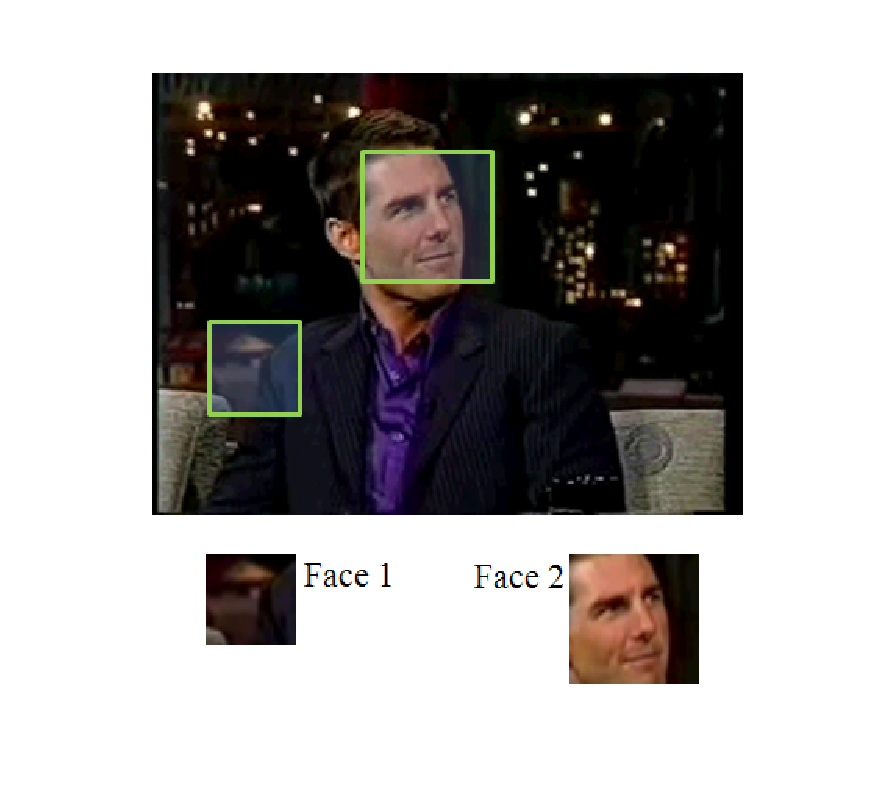
\includegraphics[width=3in]{Figure1.eps}
\caption{{\bf {\fontfamily{phv}\selectfont An example false face
detection using Viola-Jones \cite{viola_robust_2004} face detection
algorithm.}}} \label{Fig:ExampleFalseDetect}
\end{figure}

The problem of false face detection has motivated some researchers
to develop heuristic approaches aimed for validating the face
detection results. Most of these heuristics integrate primitive
context into the problem by searching for skin tone in the output
subimages. However, this simple approach often fails to distinguish
faces from non-faces, because face detectors often fail to center
the cropping box precisely around the detected face. This produces a
significant patch of skin colored pixels, but only a partial face.
This centering problem can be dealt with by extracting the skin
colored regions and comparing their shape to an ellipse. While such
heuristics, are simple, and somewhat effective, their validation is
not reliable enough to meet the needs of higher level face
processing tasks. Further, they do not provide a confidence metric
for their validation.

\begin{figure}[h]
\centering
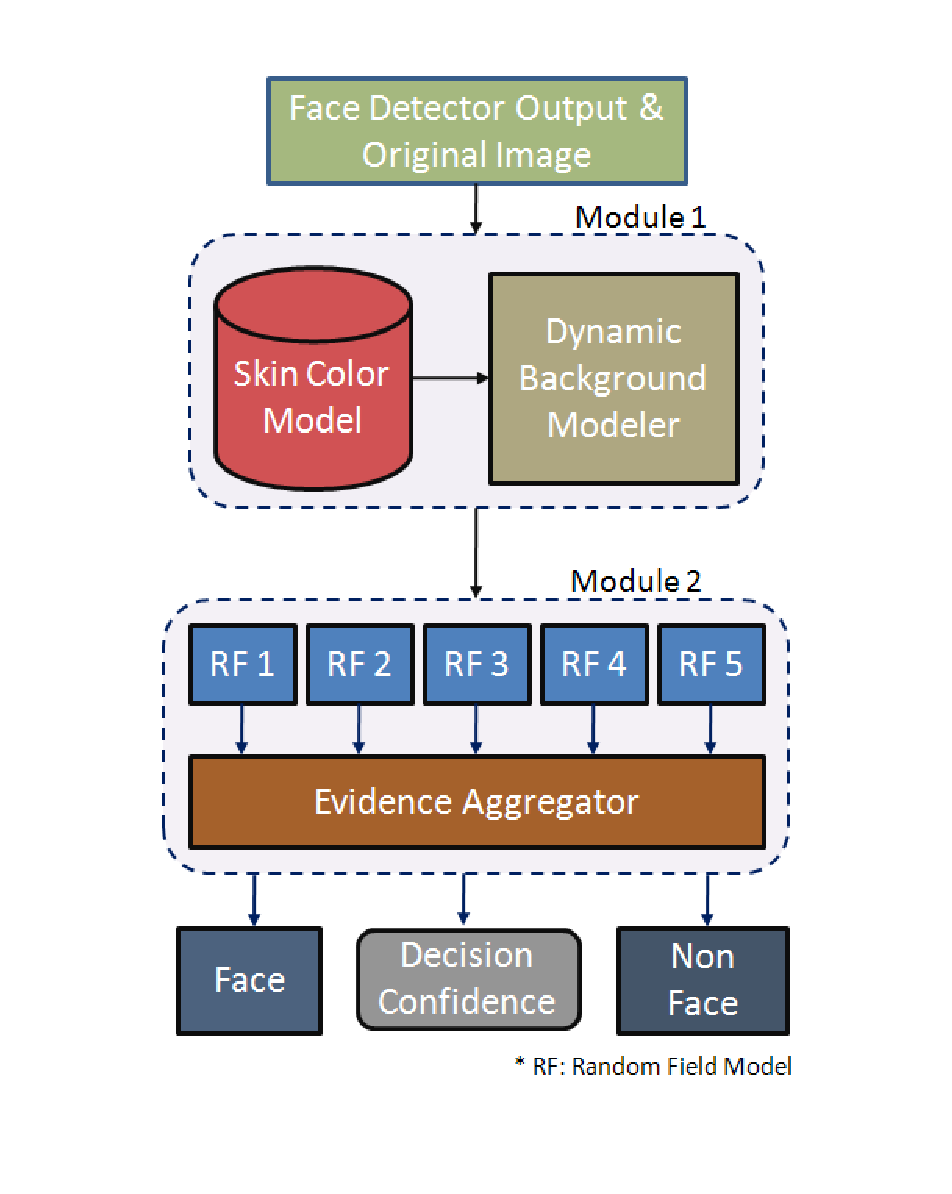
\includegraphics[width=3.5in]{Figure2.eps}
\caption{{\bf {\fontfamily{phv}\selectfont Block diagram of the
proposed framework for face detection validation.}}}
\label{Fig:BlockDiagram}
\end{figure}

This paper treats the problem of face detection validation in a
systematic manner, and proposes a learning framework that
incorporates both contextual and structural knowledge of human
faces. A face validation filter is designed by combining two
statistical modelers, 1) a human skin tone detector with a dynamic
background modeler (Module $1$), and 2) an evidence-aggregating
human face silhouette random field modeler (Module $2$), which
provides a confidence metric representing its validation of the
face. The block diagram in Figure \ref{Fig:BlockDiagram} shows the
functional flow of data through the two modules in the proposed
framework. The details of the statistical models and their learning
will be presented later in the paper, which is organized as follows.
Section 2 reviews some of the earlier research aimed at validating
face detection results. Section 3 introduces the proposed framework,
with details on the learning process. Section 4 discusses the data
used for training and testing the framework. Section 5 presents and
discusses the results, and Section 6 presents conclusions and a
discussion of future work.

%-------------------------------------------------------------------------
\Section{Related Work}\label{RelatedWork} \vspace{-0.2in} As
mentioned earlier, the problem of face detection validation has not
been treated methodically before, though the problem has been
handled by many as an integral component of face detection
algorithms. All the past work in this area can be broadly
characterized into two groups: a) Low level image feature models
mostly based on skin color such as \cite{a_hadid_hybrid_2006},
\cite{naseem_robust_2005} and \cite{m_wimmer_person_2006}, and b)
High level facial feature models such as \cite{hmid_fuzzy_2006},
\cite{tariq_face_2004} and \cite{yan-wen_wu_face_2008}.

The low level skin color based approaches try to reduce
computational complexity by first identifying skin color in images
so that search can be reduced. Most of the times, simple geometrical
properties of the retained skin regions are used to determine if the
region is a face. Such simplification of faces into trivial
geometrical structures could result in face detections. The facial
feature based methods achieves face detection by individually
identifying the integral components of a face image such as eyes,
nose, etc. Though these schemes could be robust, the associated
computational load is high. Interested readers could find more
related references in \cite{ming-hsuan_yang_detecting_2002} and
\cite{hjelm�s_face_2001}.

%-------------------------------------------------------------------------
\Section{Proposed Framework}\label{ProposedFramework}
\vspace{-0.2in} As Shown in Figure \ref{Fig:BlockDiagram}, the
framework essentially has two statistically learnt models, Module
$1$ and Module $2$, that are cascaded to form the face detection
validation filter. The output from a face detector is sent to Module
$1$, which distinguishes the skin pixels in the face region from the
background pixels, thereby constucting a skin region mask. This skin
region mask then becomes the input to Module $2$, which is
essentially an aggregate of random field models learnt from manually
labeled ({\it true}) face detection outputs. The results of each
random field model within the aggregate are then combined, using
rules of Dempster-Shafer Theory of Evidence
\cite{sentz_combination_2002}. This {\it combining of evidence}
provides a metric for the belief (i.e. confidence) of the system in
its final validation. The two modules are detailed in the following
subsections.
%-------------------------------------------------------------------------
\SubSection{Module $1$: Human Skin Tone Detector with Dynamic
Background Modeler}\label{Module1} \vspace{-0.2in} Most of the skin
tone detectors used for human skin color classification use prior
knowledge, which is provided in the form of a parametric or
non-parametric model of skin samples that are extracted from images
- either manually, or through a semiautomated process. In this paper
we employ such an a priori model, in combination with a dynamic
background modeler, so that the skin vs. non-skin boundary is
accurately determined. Accurate skin region extraction is essential
for Module $2$, as it validates images based on their structural
properties. The two functional components of Module $1$ are:

\subsubsection{{\em a-priori} Bi-modal Gaussian Mixture Model
for Human Skin Classification}\label{Bi-ModGaussian} A normalized
RGB color space has been a popular choice among researchers for
parametric modeling of human skin color. The normalized RGB
(typically represented as nRGB) of a pixel $X$ with $X_r$, $X_g$,
$X_b$ as its red, green and blue components respectively, is defined
as:
\begin{equation}
X_{i|i \in \{r,g,b\}}^{nRGB} =
\frac{X_i}{\left(\sum\limits_{\forall_{i|i\in\{r,g,b\}}}X_i\right)}
\end{equation}
Normalized RGB space has the advantage that only two of the three
components, nR, nG or nB, is required at any one time to describe
the color. The third component can be derived from the other two as:
\begin{equation}
X_{i|i \in \{nR,nG,nB\}}^{nRGB} =  1 -\left(
\sum_{\forall_{k|(k\in\{nR,nG,nB\}, k \ne i)}}X_k \right)
\end{equation}

\vspace{-0.15in}
\begin{figure}[h]
\centering
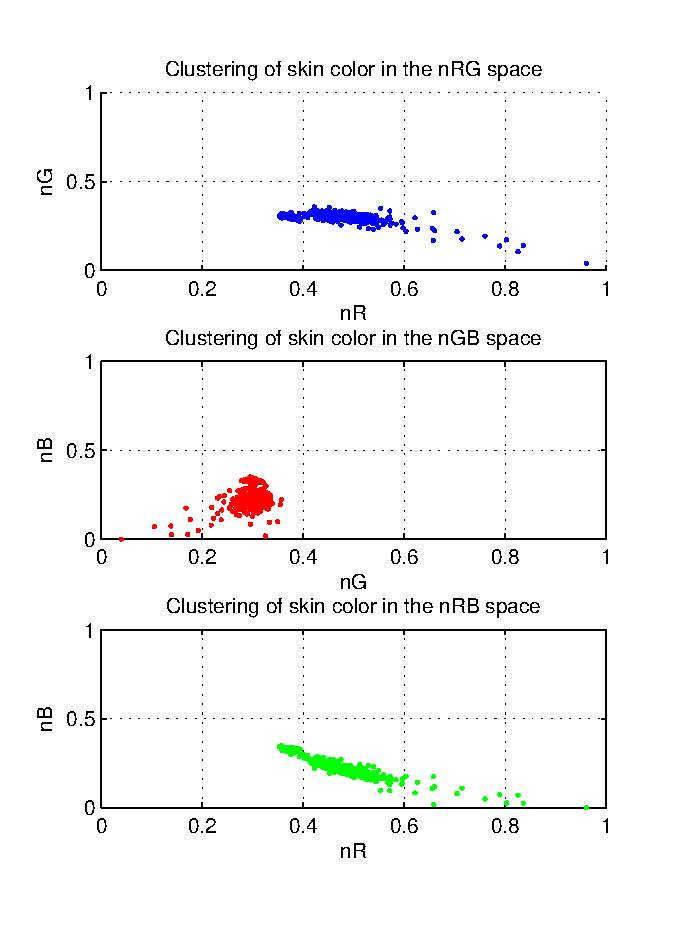
\includegraphics[width=3in]{Figure3.eps}
\caption{{\bf {\fontfamily{phv}\selectfont Projection of 1000
randomly sampled skin samples in three different nRGB spaces.\\}}}
\label{Fig:nRGBProject}
\end{figure}

In our experiments, we found that skin pixels form a tight cluster
when projected on nG and nB space as shown in the Figure
\ref{Fig:nRGBProject}. The study was based on a skin pixel database,
consisting of nearly $150,000$ samples, built by randomly sampling
skin regions from $1040$ face images collected on the web as well as
from FERET face database \cite{phillips_feret_1997}. Further
analysis also showed that the cluster formed on the 2D nG-nB space
had two prominent density peaks which motivated the modeling of skin
pixels with a Bi-modal Gaussian mixture model learnt using
Expectation Maximization (EM) with a $k$-means initialization
algorithm \cite{bilmes_gentle_1998}. The final modal is shown in
Figure \ref{Fig:BimodGaussian}. For the sake of completeness, we
provide the parameters of Bi-modal Gaussian mixture which was used
in our experiments.
\begin{eqnarray}
f^{skin}_{X|X=[nG,nB]}(x) & = & w_1 f_{Y_1}(x;\Theta_1=[\mu_1,\Sigma_1]) +  \nonumber  \\
       &  & w_2 f_{Y_2}(x;\Theta_2=[\mu_2,\Sigma_2])
\end{eqnarray}
where, $w_1 = 0.76$, $w_2 = 0.24$, $\mu_1 = [0.30,0.22]$, $\mu_2 =
[0.3, 0.32]$, $\Sigma_1=\left[ \begin{array}{cc} 0.024 & 0
\\ 0.017 & 0.03\end{array}\right]$, $\Sigma_2=\left[ \begin{array}{cc} 0.007 & 0
\\ -0.0016 & 0.0058\end{array}\right]$
\vspace{-0.15in}
\begin{figure}[h]
\centering
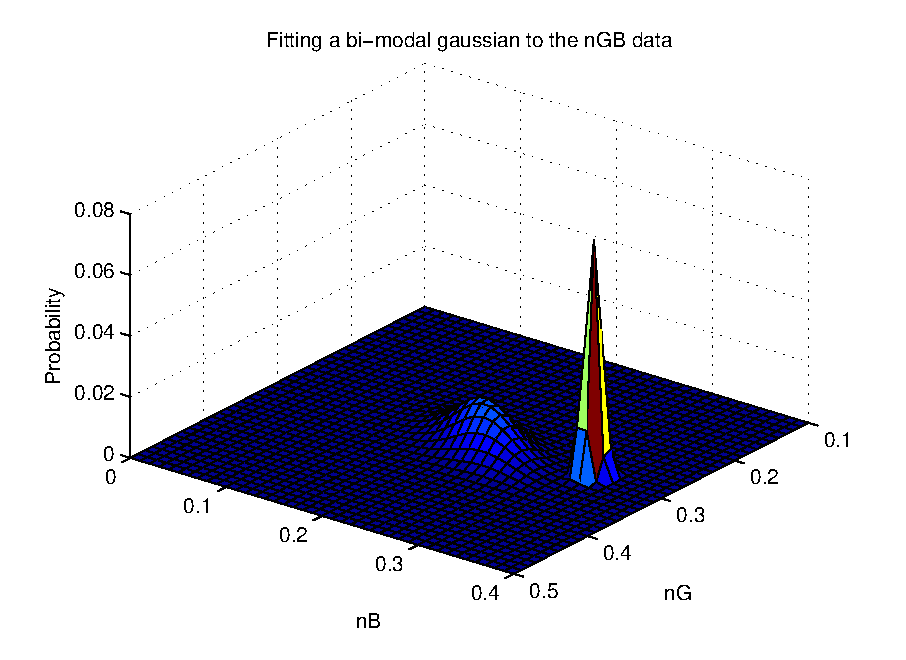
\includegraphics[width=3.5in]{Figure4.eps}
\caption{{\bf {\fontfamily{phv}\selectfont \\ Bi-modal Gaussian
fitting to skin color pixels on a nG-nB space}}}
\label{Fig:BimodGaussian}
\end{figure}
\subsubsection{Dynamically Learnt Multi-modal Gaussian Model for
Background Pixel Classification}\label{DynamicModel} As mentioned
earlier, classification of regions into face or non-face regions
requires accurate skin vs. non-skin classification. In order to
achieve this, we learn the background color surrounding each face
detector output dynamically. To this end we extract an extra region
of the original image around the face detector's output, as shown in
Figure \ref{Fig:Extraregion}. Since the size of the face detector
output varies from image to image, it is necessary to normalize the
size. This is done by downsampling the size of the original image,
to produce a face detector output region containing 90x90 pixels.
The extra region pixels surrounding the face are then extracted from
the 100x100 region around this 90x90 normalized face region.

\begin{figure}[h]
\centering
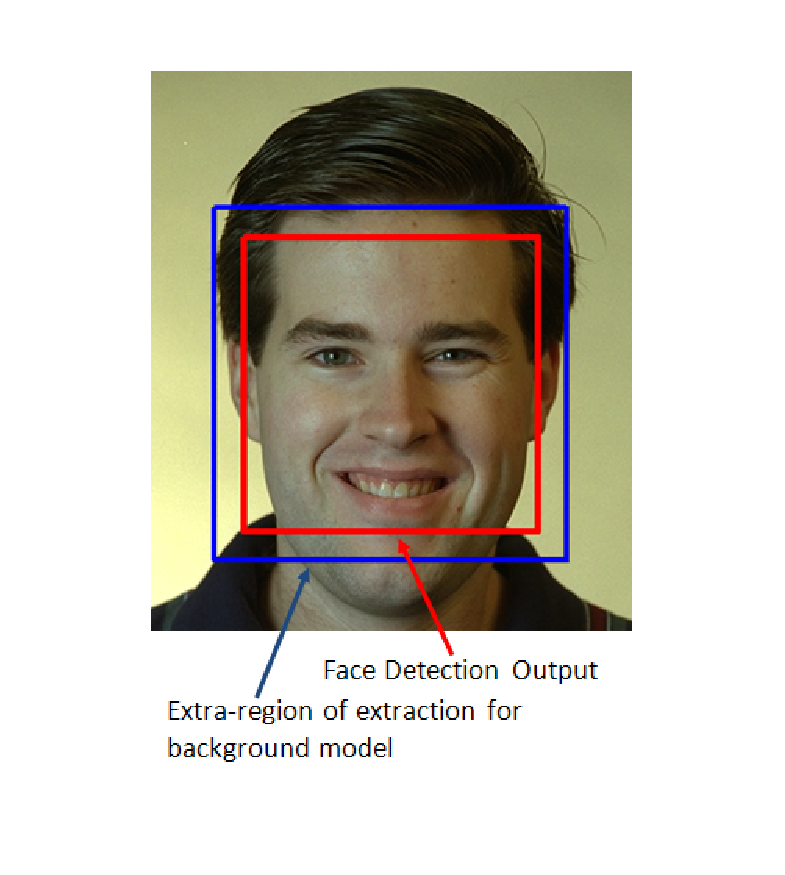
\includegraphics[width=2.5in]{Figure5.eps}
\caption{{\bf {\fontfamily{phv}\selectfont Extraction of extra
region around the face detector output to learn the background
model.}}} \label{Fig:Extraregion}
\end{figure}

Once the outer pixels are extracted, a Multi-modal Gaussian Mixture
is trained using EM with $k$-means initialization, similar to the
earlier case with skin pixel model. The resultant model can be
represented as.
\begin{equation}
f^{non-skin}_{X|X=[R,G,B]}(x) =
\sum\limits_{i=1}^{m}w(i)f_{Y_i}\left(x;\Theta_i=[\mu_i,\Sigma_i]\right)
\end{equation}
where, $m$ is the number of mixtures in the model. We found
empirically that a value of $m=2$ or $m=3$ modeled the backgrounds
with sufficient accuracy.

\subsubsection{Skin and Background Classification using the learnt
Multi-modal Gaussian Models}\label{SkinnBackground} The skin and
non-skin models, $f^{skin}_{X|X=[nG,nB]}(x)$ and
$f^{non-skin}_{X|X=[R,G,B]}(x)$ respectively, are used for
classifying every pixel in the scaled face image obtained as
explained in the Section \ref{DynamicModel}. An example skin-mask is
shown in Figure \ref{Fig:Skinmasks}. This example shows two sets of
images - one corresponding to a {\it true} face detection result,
and another {\it false} face detection result. \vspace{-0.15in}
\begin{figure}[h]
\hspace{-0.4in}
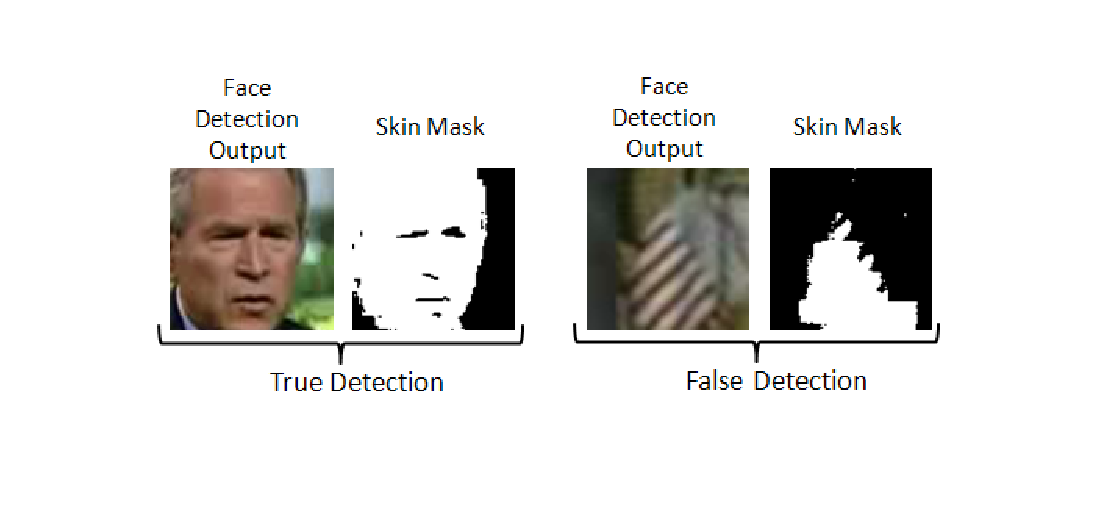
\includegraphics[width=4in]{Figure6.eps}
\caption{{\bf {\fontfamily{phv}\selectfont Example of {\em true} and
{\em false} face detection results with their corresponding skin
masks extracted as explained in Section \ref{DynamicModel}}}}
\label{Fig:Skinmasks}
\end{figure}
The structural analysis through Random Field models explained in the
next section will describe the design concepts that will help
distinguish between {\it true} and {\it false} face detections shown
in Figure \ref{Fig:Skinmasks}.
%-------------------------------------------------------------------------
\SubSection{Module $2$: Evidence-Aggregating Human Face Silhouette
Random Field Modeler}\label{Module2} \vspace{-0.2in}
 The structural analysis through
Random Field models detailed in this section will describe how the
evidence arrogator is used to distinguish between the {\it true} and
{\it false} face detections shown in Figure
\ref{Fig:ExampleFalseDetect}. In order to validate the skin region
extracted as explained in Section \ref{Module1}, we build
statistical models from examples of faces. We developed statistical
learners inspired by Markov Random Fields (MRF) to capture the
variations possible in {\it true} skin masks (face silhouette). The
following subsections describes MRF models and the variant we
created for our experiments.

\subsubsection{Random Field (RF) Models}\label{MRF} MRFs encompass a
class of probabilistic image analysis techniques that rely on
modeling the intensity variations and interactions among the image
pixels. MRFs have been widely used in low level image processing
including, image reconstruction, texture classification and image
segmentation \cite{perez_markov_1998}. In this work, we use MRFs to
learn the structure of a {\it true} face skin mask.

In an MRF, the sites in a set, $\mathcal S$, are related to one
another via a neighborhood system, which is defined as ${\mathcal
N}=\{{\mathcal N}_i, i \in \mathcal S\}$, where ${\mathcal N}_i$ is
the set of sites neighboring $i$, $i \notin {\mathcal N}_i$ and $i
\in {\mathcal N}_j \Longleftrightarrow j \in {\mathcal N}_i$.

A random field X said to be an MRF on $\mathcal S$ with respect to a
neighborhood system $\mathcal N$, if and only if,
\begin{eqnarray}&& P({\mathbf x})>0, \forall \mathbf x \in \mathcal X  \\ && P(x_i\vert x_{{\mathcal S}-\{i\}})=P(x_i\vert x_{{\mathcal N}_i}) \label{Eqn:5} \end{eqnarray}
where, $P(x_i\vert x_{{\mathcal S}-\{i\}})$ represents a Local
Conditional Probability Density function defined over the
neighborhood $\mathcal N$. The variant of MRF that we created for
our experiments relaxed the constraints imposed by MRFs on $\mathcal
N$. Typically, MRFs requires that sites in set $\mathcal S$ be
contiguous neighbors. The relaxation in our case allows for distant
sites to be grouped into the same model.

We empirically found out that modeling the skin-region validation
problem into one single RF gave poor results. We devised $5$ unique
RF models with an Dempster-Shafer Evidence aggregating framework
that could not only validate the face detection outputs, but also
provide a metric of confidence. Thus, Equation \ref{Eqn:5} could be
alternatively seen as a set $P({\mathbf x}) = \{P^1({\mathbf x}),
\ldots, P^5({\mathbf x})\}$, each having their own neighborhood
system $\mathcal N^k = \{\mathcal N^1, \mathcal N^2, \ldots,
\mathcal N^5\}$, such that
\begin{equation}
P^k(x_i\vert x_{{\mathcal S}-\{i\}})=P(x_i\vert x_{{\mathcal
N^k_i}})
\end{equation}

\subsubsection{Pre-processing}\label{Preprocessing}As described earlier,
each face detector output is normalized and expanded to produce a
$100$x$100$ pixel image, from which a binary skin mask is generated.
A morphological opening and closing operation is then performed on
the skin mask (to eliminate isolated skin pixels), and the mask is
then partitioned into one hundred $10$x$10$ blocks, as shown in
Figure \ref{Fig:RowColumnBlocks}. The number of mask pixels (which
represent skin pixels) are counted in each block, and a $10$x$10$
matrix is constructed, where each element of this matrix could
contain a number between 0 and 100. This $10$x$10$ matrix is then
used as the basis for determining whether the face detector output
is indeed a face.

\begin{figure}[h]
\hspace{-0.3in}
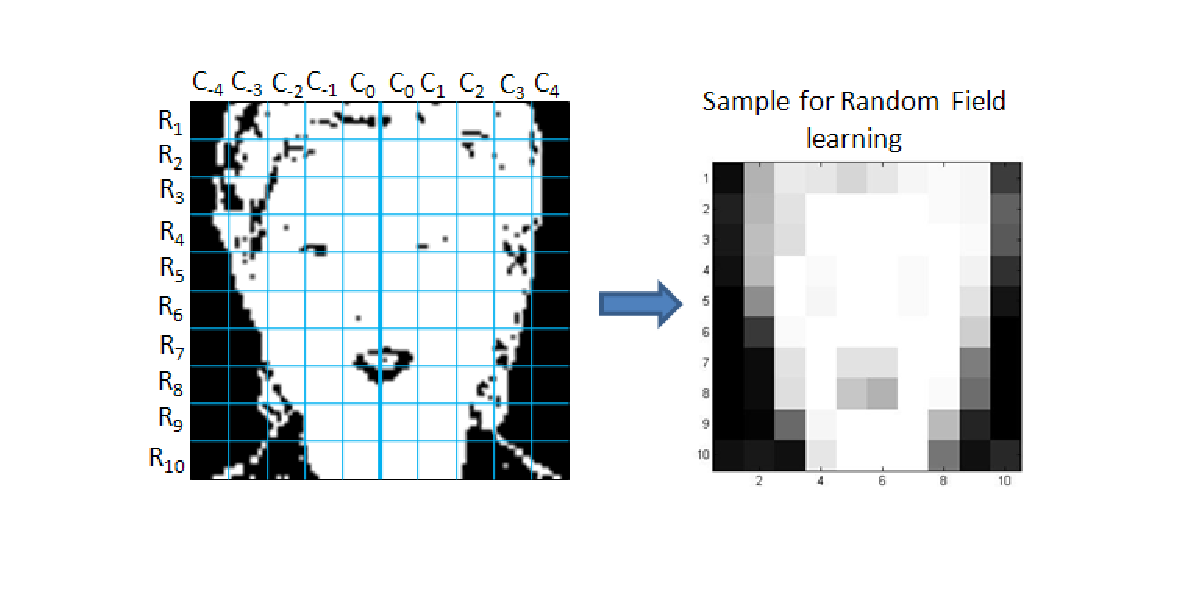
\includegraphics[width=4in]{Figure7.eps} \caption{{\bf
{\fontfamily{phv}\selectfont Pre-processing of skin-region mask
generated from Module 1.}}} \label{Fig:RowColumnBlocks}
\end{figure}

\subsubsection{The Neighborhood System}\label{Neighborhood}The determination of whether the
face detector output is actually a face is based on heuristics that
are derived from anthropological human face models
\cite{vezjak_anthropological_1994} and through our own statistical
analysis. These include:
\begin{enumerate}
\item Human faces are horizontally symmetrical (i.e. along any row of blocks $R_i$)
about a  central vertical line joining the nose bridge, the tip of
the nose and the chin cleft, as shown in Figure
\ref{Fig:RowColumnBlocks}.  In particular, our analysis of a large
set of frontal face images showed that the counts of skin pixels in
the 10 blocks that form each row in Figure \ref{Fig:RowColumnBlocks}
were roughly symmetrical across this central line.

\item The variations along the verticals ($C_i$'s) are negligible enough
that in building a Local Conditional Probability Density function,
each $R_i$ can be considered independent of the other. That is, for
example, modeling variations of $C_0$ w.r.t $C_1$ on $R_1$ is
similar to modeling variations of $C_0$ w.r.t $C_1$ on any other
$R_{i|i\ne1}$. Thus, analysis of Local Conditional Probability could
be restricted to single $R_i$ at a time, as shown in Figure
\ref{Fig:Neighborhood}.
\end{enumerate}

\begin{figure}[h]
\hspace{-0.3in}
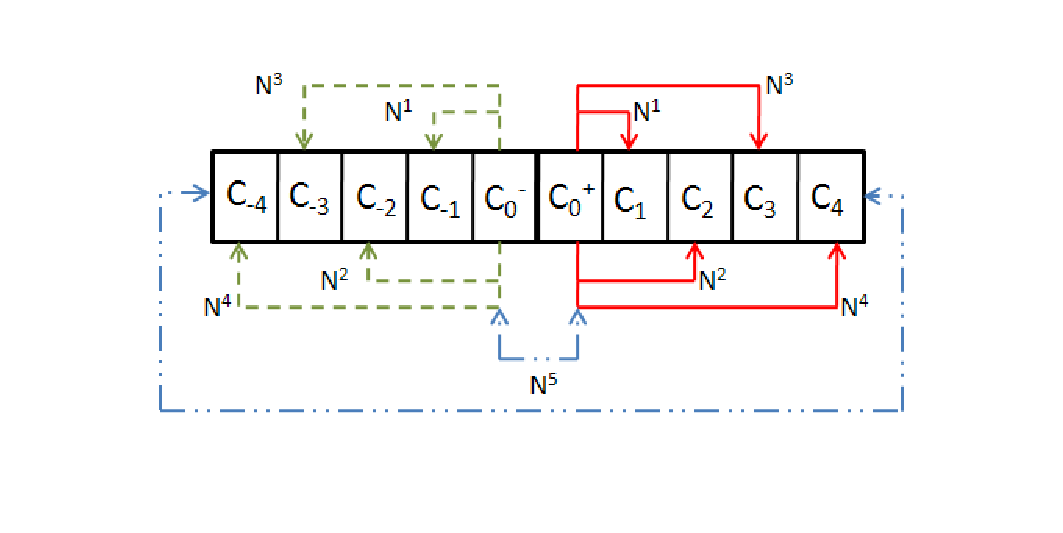
\includegraphics[width=4in]{Figure8.eps} \caption{{\bf
{\fontfamily{phv}\selectfont Neighborhood System chose for our
Random Field (RF) models.}}} \label{Fig:Neighborhood}
\end{figure}

The different neighborhood systems $\mathcal N^k$, used in the RF
models, $P^k(x\vert x_{\mathcal N}^k)$, can be defined as (Refer
Figure \ref{Fig:Neighborhood}):
\begin{equation}
\mathcal N^k = \left\{C_{j | j \in \{|k|, 0^-, 0^+\}}\right\}
\end{equation}

\subsubsection{Local Conditional Probability Density (LCPD)}\label{LCPD} To model the
variations on the skin-region mask, we choose to build 2D histogram
for each of the $5$ RF over their unique neighborhood system. The
design of the dimensions were such that they captured the various
structural properties of {\it true} skin masks. The two dimensions
(represented in a histogram pool ${\mathbf H}^k$) with individual
element of the pool, ${\mathbf z}$, can be defined as:
\begin{itemize}
\item $\mathbf{H}^{k|k=\{1,2,3,4\}} = \left\{ \mathbf{z}\right\}$, where,
\begin{equation}\mathbf{z} = [x_{C_{0^{\pm}}}, \delta(x_{C_{0^{\pm}}},
x_{C_{\pm k}})] , \forall R_{j} \label{Eqn:9}
\end{equation}

\item$\mathbf{H}^{k=5} = \left\{
\mathbf{z}\right\}$, where,
\begin{equation}
\mathbf{z} = [\mu(x_{C_{0^+}},x_{C_{0^-}}), \mu(x_{C_{-4}},
x_{C_{+4}})] , \forall R_{j} \label{Eqn:10}
\end{equation}
\end{itemize}

where, $x_{C_k}$ is the count of skin pixels in the block $C_k$. The
two functions $\delta(.,.)$ and $\mu(.,.)$ are defined as
\begin{eqnarray}
\delta(x_{C_{0^{\pm}}}, x_{C_{\pm i}}) & = & \left\{
\begin{array}{l l}
x_{C_{0^+}} - x_{C_{+i}}, & i>0 \\
x_{C_{-i}} - x_{C_{0^-}}, & i<0 \\
\end{array}
\right. \\
\mu(a,b) & = & \frac{a+b}{2}
\end{eqnarray}
In order to estimate the LCPD on these $5$ histogram pools, we use
Parzen Window Density Estimation (PWDE) technique, similar to
\cite{paget_texture_1997}, with a 2D Gaussian window. Thus, each of
LCPD can now be defined as
\begin{eqnarray}
 P^k(\mathbf z) = {\mathcal A} \sum\limits_{j=1}^n \exp
\left[-\frac{1}{2 h^2_{opt}} \left(\mathbf{z} - \mathbf
{H}^k_j\right)^T \Sigma^{-1} \left( \mathbf{z} - \mathbf
{H}^k_j\right) \right],   \\ \hspace{-1in}{\mathcal A} =
\frac{1}{(2\pi)^{\frac{d}{2}} n h_{opt}^d} \nonumber
\end{eqnarray}

where, $n$ is the number of samples in the histogram pool
$\mathbf{H}^k$, $d$ is number of dimensions (in our case $2$),
$\Sigma$ and $h_{opt}$ are the covariance matrix over $\mathbf{H}^k$
and the optimal window width, respectively, defined as:
\begin{eqnarray}
\Sigma = \left[\begin{array}{cc} \sigma_{dim1} & 0 \\ 0 &
\sigma_{dim2}\end{array} \right], & h_{opt} =
\frac{\sigma_{dim1}+\sigma_{dim2}}{2} \left\{\frac{4}{n(2d+1)}
\right\}^{1/(d+4)}          \nonumber
\end{eqnarray}
Figure \ref{Fig:LCPDs} shows the $5$ LCPDs learnt over a set of
$390$ training frontal face images.
\begin{figure}[h]
\hspace{-0.3in}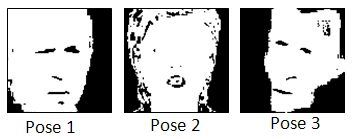
\includegraphics[width=4in]{Figure9.eps}
\caption{{\bf {\fontfamily{phv}\selectfont The $5$ Local Conditional
Probability Density (LCPD) models for learnt of set of frontal
skin-region masks.}}} \label{Fig:LCPDs}
\end{figure}
\subsubsection{Human Face Pose}\label{HumanFacePose}During our studies we discovered that
the structure of the skin-region varies based on the pose of
detected face as shown in Figure \ref{Fig:PoseMasks}. Combining face
examples from different pose into one set of RFs seemed to dilute
the LCPDs and hence the discriminating capability. This motivated us
to design three different sets of RFs, one for each pose. This was
accomplished by grouping {\it true} face detections into three
piles, Turned right ($r$), Facing front ($f$), and, Turned Left
($l$).
\begin{figure}[h]
\hspace{-0.3in}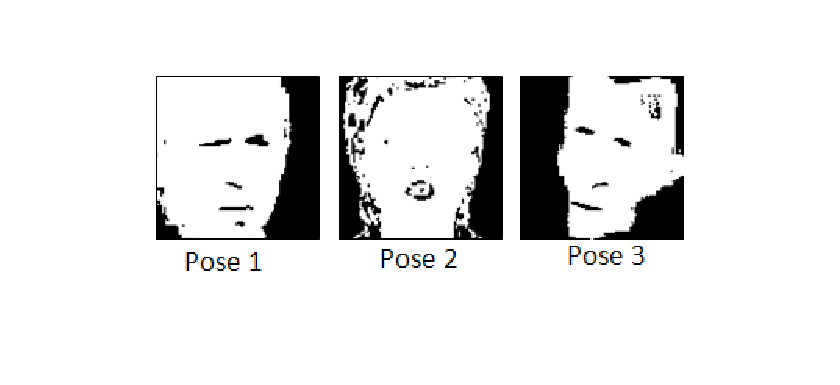
\includegraphics[width=4in]{Figure10.eps}
\caption{{\bf {\fontfamily{phv}\selectfont Skin-region masks for
three pose groups used in our experiments.}}} \label{Fig:PoseMasks}
\end{figure}
Thus, the final set of LCPDs could be described by the super set.
\begin{equation}
P(\mathbf z) = \left\{P^{k|k=\{1,\ldots,5\}}_{m|m=\{r,f,l\}}(\mathbf
z) \right\}
\end{equation}

\subsection{Combining Evidence}\label{CombiningEvidence}
\vspace{-0.2in} Given any test face detection output, $\mathbf{z}$
is extracted (as described in Equation \ref{Eqn:9} and \ref{Eqn:10})
and projected on the LCPD set $P(\mathbf z)$ to get a set of
likelihoods $l_m^k$. As in the case of any likelihood analysis, we
combined the joint likelihood of multiple projections using
log-likelihood function, $L_m^k = \ln \left(l_m^k\right)$, such
that,
\begin{equation}
\prod\limits_{\forall {\mathbf z} \in {\mathbf H}^k_m}\ln
\left(l_m^k(\mathbf z)\right) =  \sum\limits_{\forall {\mathbf z}
\in {\mathbf H}^k_m}L_m^k(\mathbf z)
\end{equation}
Given these log-likelihood values, one can set hard thresholds on
each one of them to validate a face subimage discretely as {\it
true} or {\it false}. We incorporated a piece-wise linear decision
model (soft threshold) instead of a hard threshold on the acceptance
of a face subimage. This is illustrated in the Figure
\ref{Fig:Thresholds}. Each LCPD $P^k(\mathbf z)$ was provided with
an upper and lower threshold of acceptance and rejection
respectively. The upper and lower bounds were obtained by observing
$P^k(\mathbf z)$ for the three face poses $P^k_{r,f,l}(\mathbf z)$.
Thus, any log-likelihood values lesser than the lower threshold
($L_L$) would result in a decision against the test input
(Probability $0$), while any log-likelihood value greater that the
upper threshold ($L_U$) would be a certain accept (probability $1$).
Anything in between would be assigned a probability of acceptance.
\begin{figure}[h]
\centering
\hspace{-0.3in}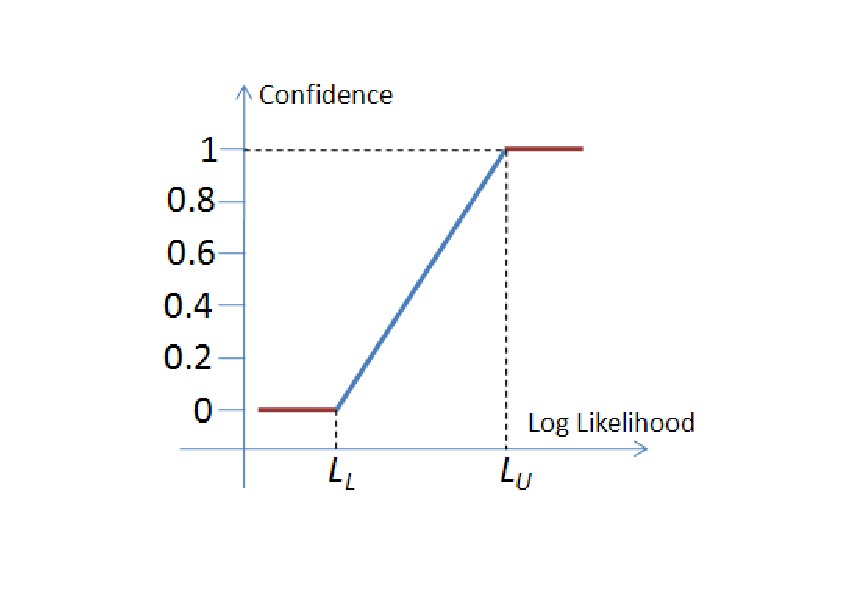
\includegraphics[width=2.5in]{Figure11.eps}
\caption{{\bf {\fontfamily{phv}\selectfont Soft threshold limits on
log-likelihood values.}}} \label{Fig:Thresholds}
\end{figure}
In order to combine the decisions from the five LCPD $P^k(\mathbf
Z)$, we resort to Dempster-Shafer Theory of Evidence.

\subsubsection{Dempster-Shafer Theory of Evidence (DST)}\label{DST}
The Dempster-Shafer theory is a mathematical theory of evidence
\cite{sentz_combination_2002} which is a generalization of
probability theory with probabilities assigned to sets rather than
single entities.

If $X$ is an universal set with power set, $\mathbf{P}(X)$ (Power
set is the set of all possible sub-sets of $X$, including the empty
set $\emptyset$), then the theory of evidence assigns a belief mass
to each subset of the power set through a function called the basic
belief assignment (BBA), $m:\mathbf{P}(X) \rightarrow [0,1]$, when
it complies with the two axioms. a) $m(\emptyset) = 0 $ and b)
$\sum\limits_{\mathbf{A} \in \mathbf{P}(X)} m(\mathbf{A})= 1$. The
mass, $m(A)$, of a given member of the power set expresses the
proportion of all relevant and available evidence that supports the
claim that the actual state belongs to $A$ and to no particular
subset of $A$. In our case, $m(A)$ correlates to the probability
assigned by each of  LCPDs towards the subimage being a face or not.

The true use of DST in our application becomes clear with the {\it
rules of combining evidences} which was proposed as an immediate
extension of DST. The combined mass (evidence) of any two experts
opinions, $m_1$ and $m_2$, can be represented as:
\begin{equation}
m_{1,2}(A) = \frac{1}{1-K}\sum\limits_{B\cap C = A, A \ne
\emptyset}m_1(B) m_2(C) \label{Eqn:16}
\end{equation}
where,
\begin{equation}
K = \sum\limits_{B \cup C = \emptyset}m_1(B) m_2(C) \label{Eqn:17}
\end{equation}is a measure of the conflict in the experts opinions. The
normalization factor, $(1-K)$, has the effect of completely ignoring
conflict and attributing any mass associated with conflict to a null
set.

The $5$ LCPDs, $P^k(\mathbf z)$, were considered as experts towards
voting on the test input as a face or non-face. In order to use
these mapped values in Equation \ref{Eqn:16} - \ref{Eqn:17}, we
normalized evidences generated by the experts to map between
$[0,1]$, and any conflict of opinions were added into the conflict
factor, $K$. For the sake of clarity, we show an example of
combining two expert opinions in Figure \ref{Fig:DST}. The same idea
could be extended to multiple experts.
\begin{figure}[h]
\centering
\hspace{-0.2in}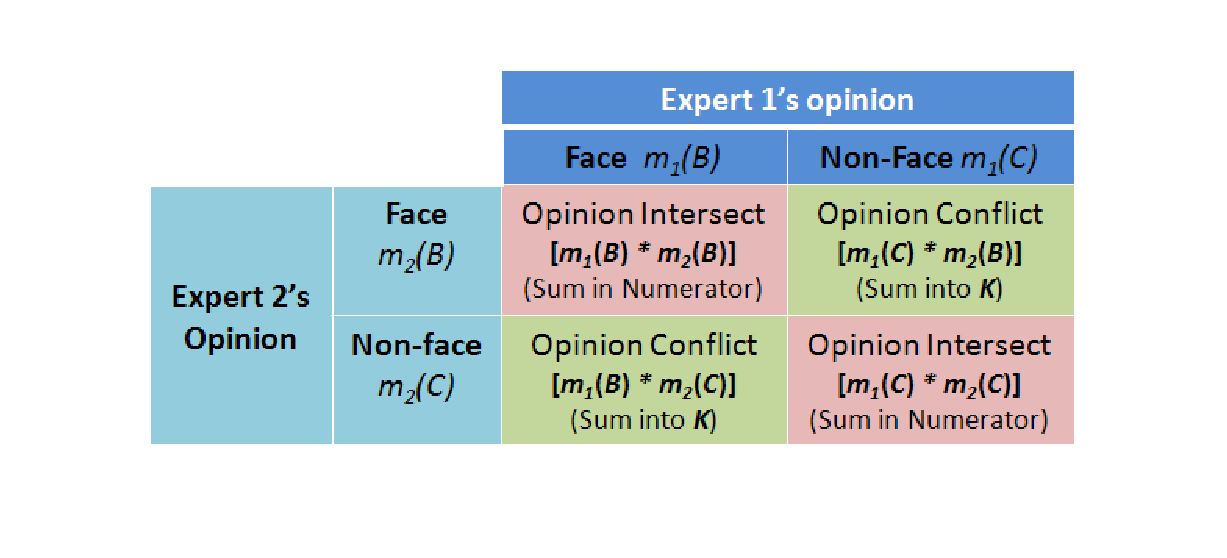
\includegraphics[width=3.5in]{Figure12.eps}
\caption{{\bf {\fontfamily{phv}\selectfont An example of combining
evidence from two experts under Dempster-Shafer Theory.}}}
\label{Fig:DST}
\end{figure}

\subsection{Coarse Pose estimation}\label{CoarsePoseEstimation}
\vspace{-0.2in} Since the RF models were biased with pose
information, we also investigated the possibility of determining the
pose of the face based on the evidences obtained from the LCPDs. We
noticed that the LCPDs $P^3(\mathbf z)$, $P^4(\mathbf z)$ and
$P^5(\mathbf z)$ were capable of not only discriminating faces from
non-faces, but were also capable of voting towards one of $3$ pose
classes, Looking right, Frontal, and Looking Left along with a
confidence metric. Due to space constraints, the procedure is not
explained in detail, but it is similar to what was followed for face
versus non-face discrimination as explained in Section
\ref{CombiningEvidence}.

%-------------------------------------------------------------------------
\Section{Experiments}\label{Experiments} \vspace{-0.2in} In all our
experiments, Viola-Jones face detection algorithm
\cite{viola_robust_2004} was used for extracting face subimages. The
proposed face validation filter was tested on two face image data
sets 1. {\it The FERET Color Face Database} and 2. {\it An in-house
face image database} created from interview videos of famous
personalities. Viola-Jones face detection algorithm
\cite{viola_robust_2004} was used in all our experiments. In order
to prepare the data for processing, face detection was performed on
all the images in both the data sets. The number of face detections
do not directly correlate to the number of unique face images as
there are plenty of false detections. We manually identified each
and every face detection to be {\it true} or {\it false} so that
ground truth could be established. The details of this manual
labeling is shown below:
\begin{enumerate}
\item {\em FERET}
\begin{itemize}
\item Number of actual face images: $14,051$
\item Number of faces detected using Viola-Jones algorithm: $6,208$
\item Number of {\it true} detections: $4,420$
\item Number of {\it false} detections: $1,788$ ($28.8$\%)
\end{itemize}
\item {In-house database}
\begin{itemize}
\item Number of actual face images: $2,597$
\item Number of faces detected using Viola-Jones algorithm: $2,324$
\item Number of {\it true} detections: $2,074$
\item Number of {\it false} detections: $250$ ($10.7$ \%)
\end{itemize}
\end{enumerate}

 %-------------------------------------------------------------------------
\Section{Results} \label{Sec:Results} \vspace{-0.2in}
 The face detections from the above mentioned data set were passed through
 the face detection validation filter, as in Figure \ref{Fig:BlockDiagram}. In order to compare the
 performance of the face validation filter, we have chosen four parameters:
 \begin{enumerate}
 \item {\bf Number of false detections (NFD)}
 \begin{equation}
\mbox{NFD} = \mbox{Count of false detections during the experiment}
\nonumber
 \end{equation}
 \item {\bf False detection rate (FDR):} \begin{equation}
 \mbox{FDR} = \frac{\mbox{\# of false detections}}{\mbox{Total \# of face
 detections}} \mbox{x} 100 \nonumber
 \end{equation}
 \item {\bf Precision (P)}
 \begin{equation}
 \mbox{P} = \frac{\mbox{\# of true detections}}{\mbox{\# of true detections} + \mbox{\# of false
 detections}} \nonumber
 \end{equation}
 \item {\bf Capacity (C)}
 \begin{equation}
 \mbox{C} = \left(\frac{\mbox{\# of true detections}}{\mbox{\# of actual faces in database}}\right) -
 \mbox{FDR} \nonumber
 \end{equation}
 \end{enumerate}

Table \ref{Tab:FERET} and \ref{Tab:Inhouse} shows the validation
results on the two data sets introduced in Section
\ref{Experiments}.

\begin{table}[h]
\centering
 \begin{tabular}{|c||c|c|}
   \hline
   % after \\: \hline or \cline{col1-col2} \cline{col3-col4} ...
    & Before Validation & After Validation \\
    \hline
    \hline
    NFD  &  $1,788$ & $208$ \\
   FDR & $28.8$ \% & $3.35$ \% \\
   P & $0.7120$ & $0.9551$ \\
   C & $0.026$ & $0.281$ \\
   \hline
 \end{tabular}
 \vspace{0.2in}
\caption{Face detection validation results on FERET database}
\label{Tab:FERET}
\end{table}

\begin{table}[h]
\centering
 \begin{tabular}{|c||c|c|}
   \hline
   % after \\: \hline or \cline{col1-col2} \cline{col3-col4} ...
    & Before Validation & After Validation \\
    \hline
    \hline
   NFB & $250$  &  $2$\\
   FDR & $10.76$ \% & $0.01$ \%\\
   P & $0.892$ & $0.999$ \\
   C & $0.691$ & $0.798$ \\
   \hline
 \end{tabular}
  \vspace{0.2in}
    \caption{Face detection validation results on the in-house face database}
   \label{Tab:Inhouse}
   \end{table}

  As explained in Section \ref{CoarsePoseEstimation}, the framework
  was extensible to perform coarse pose estimation. Figure
  \ref{Fig:Result} shows the result of passing two frames of a video
  sequence as input the face validation filter. The frames were
  extracted from a video of the same individual exhibiting arbitrary facial
  motion. The frames were $0.55$ seconds apart. As can be noticed,
  the head pose is slightly different between the two frames. The
  pose estimation results are shown below the two frames.

\begin{figure}[h]
\centering
\hspace{-0.3in}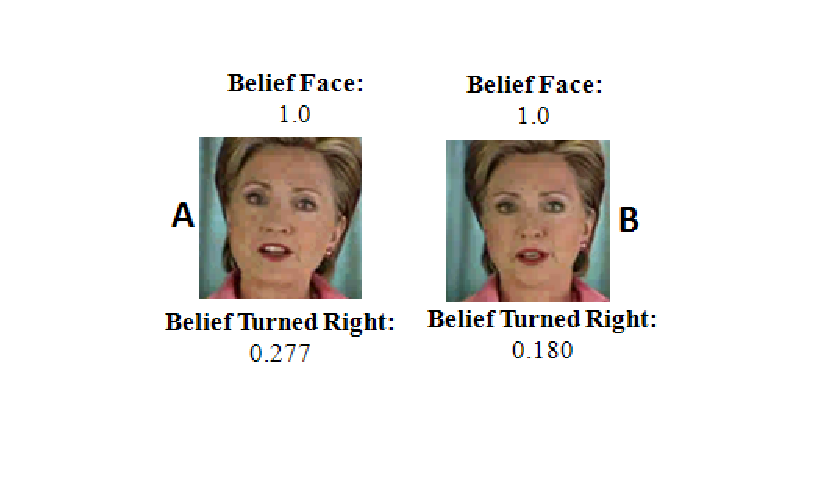
\includegraphics[width=3.5in]{Figure13.eps}
\caption{{\bf {\fontfamily{phv}\selectfont Coarse pose estimation
results from the proposed framework.}}} \label{Fig:Result}
\end{figure}

\section{Discussion of Results}
\vspace{-0.2in} Performance analysis of the proposed face validation
filter can be understood through the four parameters defined in
Section \ref{Sec:Results}. {\bf NFB} and {\bf FDR} are direct
measurements of the number of mistakes (naming non-faces as faces)
made by the face detection algorithm on the two data sets. As can be
verified from Table \ref{Tab:FERET} and \ref{Tab:Inhouse}, there is
a significant reduction in the false detections through the
introduction of the filter.

The precision parameter, {\bf P}, could be considered as the
probability that a face detection retrieved at random will truly
contain a face. It can be seen that the precision of the system
drastically improves with the introduction of the face validation
filter thereby assuring a {\it true} face sub image at the output.

The capacity parameter, {\bf C}, measures the relative difference
between face detection and false-detection rates of a face detection
system. Alternately, {\bf C} can be considered to measure the net
{\it true} face detection ability of any algorithm on a specific
face data set. {\bf C} ranges from $-1$ to $1$. $-1$ when none of
the faces in the database are detected with all reported detections
being wrong. $1$ when all the faces in the database are detected
with no false detections. It can be seen from Tables \ref{Tab:FERET}
and \ref{Tab:Inhouse} that the capacity of the face detection
system, when combined with face validation filter, is significantly
higher and moves towards $1$. One can thus infer that the combined
system has better {\it true} face detection ability.

Finally, Figure \ref{Fig:Result} shows the coarse pose estimation
results. The two frames in the figure shows cases when the face is
slightly turned right, with one ({\bf A}) turned more right than the
other ({\bf B}). The face validation filter verifies that the faces
are actually turned right and the belief values represent a scale on
the amount of rotation. Since we did not do any specific mapping of
the belief values to pose angle, we could not confirm quantitatively
how accurate the pose estimations were. Through visual consort, one
can verify that the labeling is appropriate.

%-------------------------------------------------------------------------
\Section{Conclusions and Future Work} \vspace{-0.2in} In this paper
a face detection validation filter is proposed that effectively
combines two a contextual skin color modeler and a structural face
silhouette modeler towards increased {\it true} face detection
capacity of any face detection algorithm. The proposed framework is
tested with Viola-Jones face detection algorithm on two face
databases (FERET and in-house face database) and the results confirm
the benefits of increased {\it true} face detection capacity. We
also show how the proposed framework can be used towards coarse head
pose estimation.

The work presented in this paper is part of a larger framework that
could be used to improve skin region extraction on any face image by
feeding back knowledge from the structural random field modeler into
the skin detection module. As part of future work, we plan to
migrate the static skin color model in Module 1 (see Figure
\ref{Fig:BlockDiagram}) into a dynamic skin color model which will
learn alongside the background modeler


%-------------------------------------------------------------------------
\nocite{ex1,ex2}
\bibliographystyle{latex8}
\bibliography{latex8}

\end{document}
